\documentclass[12pt,oneside]{book}
\usepackage{geometry}                		% See geometry.pdf to learn the layout options. There are lots.
\usepackage{wrapfig}				%Inclusion de Graficos al lado de Texto
\usepackage[rflt]{floatflt}				%Para meter figuras flotantes entre el texto.
\usepackage{enumerate}				%Para los items enumerados
\geometry{a4paper}                   			% ... or a4paper or a5paper or ... 
%\geometry{landscape}                		% Activate for for rotated page geometry
%\usepackage[parfill]{parskip}    		% Activate to begin paragraphs with an empty line rather than an indent
\usepackage{graphicx}				% Use pdf, png, jpg, or epsß with pdflatex; use eps in DVI mode
								% TeX will automatically convert eps --> pdf in pdflatex		
\usepackage{amssymb}

\usepackage[spanish]{babel}			% Permite que partes automáticas del documento aparezcan en castellano.
\usepackage[utf8]{inputenc}			% Permite escribir tildes y otros caracteres directamente en el .tex
\usepackage[T1]{fontenc}			% Asegura que el documento resultante use caracteres de una fuente apropiada.

\usepackage{hyperref}				% Permite poner urls y links dentro del documento
\begin{document}

\begin{titlepage}

\begin{center}
\vspace*{-1in}
\begin{figure}[htb]
\begin{center}

\includegraphics[width=8cm]{./espol}
\end{center}
\end{figure}

FACULTAD DE INGENIERIA \\
\vspace*{0.15in}
ELECTRICA Y COMPUTACIÓN \\
\vspace*{0.6in}
\begin{large}
ING: JAVIER TIBAU\\
\end{large}
\vspace*{0.4in}
\begin{Large}
\textbf{PROYECTO BUSCAMINAS EN ANDROID} \newline \newline

\begin{figure}[htb]
\begin{center}
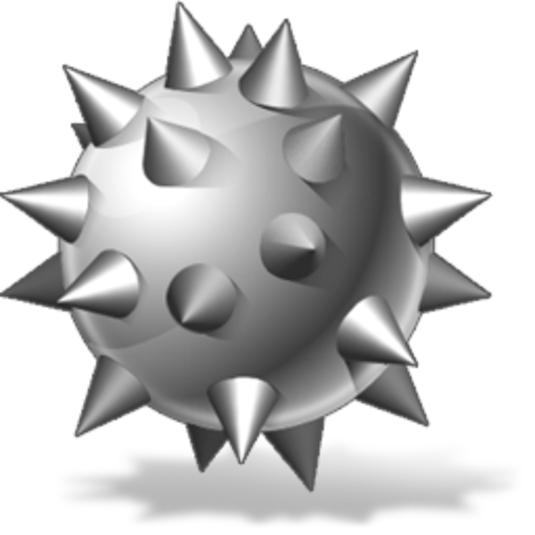
\includegraphics[width=3cm]{./icono}
\end{center}
\end{figure}

\end{Large}
\begin{large}
Integrantes:\\Leonel Ramírez\\José Vélez\\Kevin Campuzano\\ 
\end{large}
\vspace*{0.3in}
\rule{80mm}{0.1mm}\\
\vspace*{0.1in}
\begin{large}
Proyecto - Android
\end{large}
\end{center}

\end{titlepage}



\tableofcontents

\chapter{Objetivos}
Objetivos Generales
\begin{itemize}
\item Desarollar aplicaciones para dispositivos moviles con sistema operativo android.
\item Practicar la programación Orientada a Objetos.
\item Aprender a utilizar las herramientas que nos facilita el plugin de android.
\end{itemize}
Objetivos Especificos
\begin{itemize}
\item Mejorar la interfaz de usuario y aprendar el trato al Jugador.
\item Aprender el area lógica del juego.
\end{itemize}

\chapter{Derechos del Autor}
La aplicaci\'on que simula el Juego de Buscaminas que fue creada por prop\'ositos acad\'emicos como proyecto del Primer Parcial de la materia de Lenguajes de Programación que dicta el Ing. Tibau en el presente semestre <II Termino-2013>.
\\La cual fue desarrollada en conjunto por \\-José Velez \\ -Leonel Ramirez \\ -Kevin Campuzano


\chapter{Introducción}
Buscaminas es un videojuego para un solo jugador inventado por Robert Donner en 1989. El objetivo del juego es despejar un campo de minas sin detonar ninguna.\\
Este manual de usuario pretende brindar un conjunto de instrucciones al Usuario para facilitar el funcionamiento del juego BUSCAMINAS. \ \\ \\ 
Por otro lado, también brinda guías para el juego y describe las diferentes instancias que tiene el mismo. \ \\ \\
Con el fin de aprovechar al máximo la información de este documento, para ejecutar la aplicación de BUSCAMINAS el usuario debe tener en su poder un dispositivo movil que tenga instalado un Sistema Operativo Android.

\chapter{Guía del Juego}

En este capitulo explicaremos la reglas del juego BUSCAMINAS y se detallar\'a el uso del simulador del juego en las diferentes instancias que tiene el mismo. 

\section{Reglas}

El juego consiste en despejar todas las casillas de una pantalla que no oculten una mina.
\\
\begin{figure}[htbp]
\begin{center}
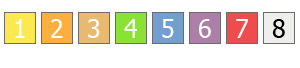
\includegraphics[width=.75\textwidth]{./imagenes/Casillas.jpg}
\caption{Casillas}
\end{center}
Algunas casillas tienen un número y color especifico, este número indica las minas que suman todas las casillas circundantes.Así, si una casilla tiene el número 3, significa que de las ocho casillas que hay alrededor (si no es en una esquina o borde) hay 3 con minas y 5 sin minas. Si se descubre una casilla sin número indica que ninguna de las casillas vecinas tiene mina y estas se descubren automáticamente.
\end{figure}
 
\ \\ 
\begin{figure}[htbp]
\begin{center}
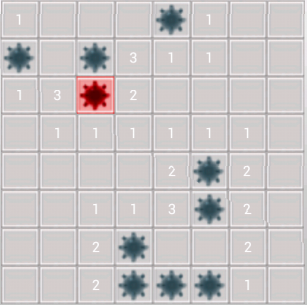
\includegraphics[width=.45\textwidth]{./imagenes/minas.png}
\caption{Perdio juego}
\end{center}
Si se descubre una casilla con una mina se pierde la partida
\end{figure}
\ \\ 
\begin{figure}[htbp]
\begin{center}

\includegraphics[width=.35\textwidth]{./imagenes/casilla_bandera.png}
\caption{Perdio juego}
\end{center}
Se puede poner una marca en las casillas que el jugador piensa que hay minas para ayudar a descubrir la que están cerca.
\end{figure}
\ \\ 
\begin{figure}[htbp]
\begin{center}
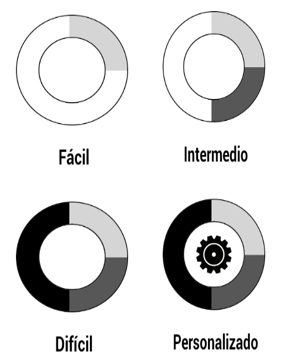
\includegraphics[width=.50\textwidth]{./imagenes/Niveles.png}
\caption{Perdio juego}
\end{center}
El juego también posee un sistema de récords para cada uno de Los 4 niveles en el que se indica el menor tiempo en terminar el juego.Los niveles son:
\\Nivel Facil: 8 x 8 casillas y 10 minas.
\\Nivel Intermedio: 10 x 10 casillas y 15 minas.
\\Nivel Dificil: 12 x 12 casillas y 20 minas.
\\Nivel Personalizado: en este caso el usuario personaliza su juego eligiendo el número de minas y el tamaño de la cuadricula.
\end{figure}

\section{Simulador}
\ \\ Al iniciar la aplicacion se mostrará un menu principal, acontinuacion explicaremos cada uno de ellos:\\

\begin{figure}[htbp]
\begin{center}
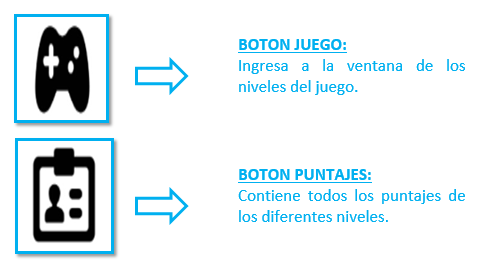
\includegraphics[width=.70\textwidth]{./imagenes/controles1.png}
\caption{Menu Principal 1}
\label{MenuPrincipal}
\end{center}
\textbf{Boton de Juego}: Este bóton es con el que se inicia a un nuevo juego, al presionar este bóton se le pedira al usuario el nivel de juego que quisisera empezar a jugar.\\
\textbf{Boton Puntajes}: Este bóton indica los records que hay por cada nivel, el record de cada jugador se graba una vez que el jugador haya ganado el juego.
\end{figure}

\begin{figure}[htbp]
\begin{center}
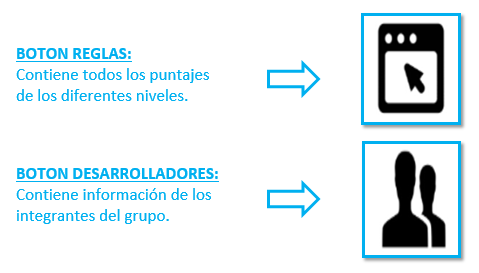
\includegraphics[width=.70\textwidth]{./imagenes/C.png}
\caption{Menu Principal 2l}
\label{MenuPrincipal}
\end{center}
\textbf{Boton Reglas}: Se indica las reglas con las que se juega, una vez empezado el juego.\\
\textbf{Boton Desarrolladores}: Presionando este boton se indican los nombres y datos adicionales de los creadores de la aplicación Buscaminas.\\
\end{figure}
\ \\ \ \\ \ \\ \ \\

\begin{figure}[htbp]
\begin{center}
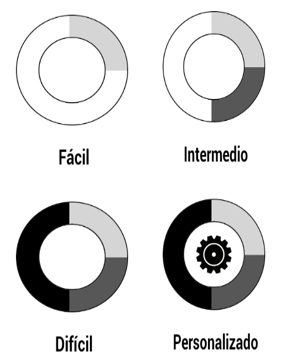
\includegraphics[width=.70\textwidth]{./imagenes/Niveles.png}
\caption{Nivel de Dificultad}
\label{Nivel de Dificultad}
\end{center}
Al presionar el bóton de Juego se le pedira al usuario escoger el nivel al que quiera empezar a jugar. Se tiene 4 niveles:
\\ \textbf{Facill} : 8 x 8  y 10 minas.
\\ \textbf{Intermedio}: 10 x 10 y 15 minas.
\\ \textbf{Dificil}: 12 x 12 y 20 minas.
\\En caso de Presionar el nivel de Dificultad: \textbf{Personalizado}: Se le pedira al jugador que eliga con que cantidad 
\\de filas, columnas y minas desea empezar a jugar.  
\end{figure} 
\ \\ \ \\ \ \\ \ \\

\begin{figure}[htbp]
\begin{center}
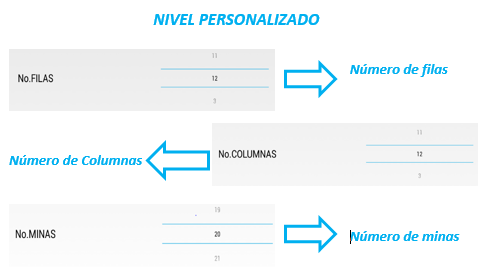
\includegraphics[width=.70\textwidth]{./imagenes/Personalizado.png}
\caption{Personalizado}
\label{Personalizado}
\end{center}
En cuanto el usuario escogio el nivel personalizado, se le pide que escoga la cantidad de filas, columnas y minas 
\\con las que el jugador quiera empezar a jugar, cabe recalcar que la cantidad de minas depende de las filas y columnas
\\con las que quiera jugar, es decir la cantidad de minas no puede ser mayor al número de celdas que se encuentren en
\\el juego. 
\end{figure} 
\ \\ \ \\ \ \\ \ \\

\begin{figure}[htbp]
\begin{center}
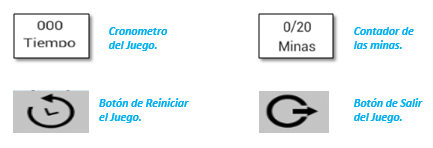
\includegraphics[width=.70\textwidth]{./imagenes/botonesR.png}
\caption{Botones en Ventana de juego}
\label{Juego}
\end{center}
En la Ventana de Juego tenemos las siguientes caracteristicas:
\\Cronometro del Juego: Indica el Tiempo que se lleva jugando la partida, cabe indicar que este tiempo solo marca en \\segundos
\\Contador de las minas: Indica la cantidad de banderas que debemos de colocar en la que suponemos que se encuentra
\\una mina, esto es una ayuda para el jugador.
\\Botón de reiniciar el juego: Presionando este bóton se reinicia el juego, indicamos que no será el mismo juego que
\\anteriormente lo jugaba.
\\Botón de Salir del Juego: Presionandolo saldremos del juego, es decir la aplicacion se cerrará.
\end{figure} 
\ \\ \ \\
\begin{figure}[htbp]
\begin{center}
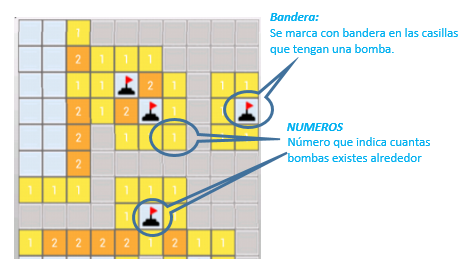
\includegraphics[width=.70\textwidth]{./imagenes/Tabla1.png}
\caption{Juego}
\label{Juego}
\end{center}
Para descubrir una celda se la presiona, en el cual se descubre si es o no una mina, en caso de que no sea mina
\\ al descubrir se indicara la cantidad de minas que esa celda tenga alrededor de ella.
\\Para marcar la celda se debe de mantener presionada alrededor de 2 segundos, hasta que la celda tome la figura
\\de una bandera de color rojo.
\end{figure} 
\ \\ \ \\
\begin{figure}[htbp]
\begin{center}
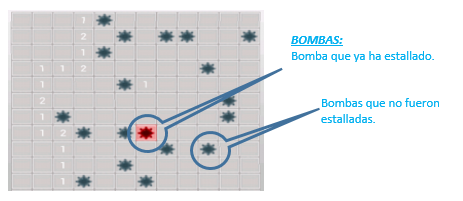
\includegraphics[width=.70\textwidth]{./imagenes/Tabla2.png}
\caption{Juego Perdido}
\label{Juego Perdido}
\end{center}
Una vez que se descubre a una mina, el jugador pierde la partida. En el tablero se resalta la mina que exploto
\\y se descubren todas las minas del tablero.
\end{figure} 

\chapter{Preguntas Frecuentes}

\begin{center}
\textbf{¿Al escoger la opción salir mientras estoy jugando una partida, la partida se guarda automaticamente?} \\ No, una partida solo se guarda el puntaje una vez ganado el juego.
\ \\ \ \\ \ \\

\textbf{¿Puedo parar el tiempo en algún instante de la partida?} \\ No, el tiempo se inicia automaticamente cuando se inicia la partida y solo se detiene al finalizar la misma.
\end{center}



\chapter{Casos de Usos}
\section{Casos de Uso}


\begin{enumerate}
	\item {Escoger opción del menú juego}
	\item {Escoger opción reglas}	
	\item{Escoger opción desarrolladores}
	\item{Escoger opción puntaje}
\end{enumerate}

\section{Caso}Escoger  opción del menú juego.\newline\newline
Descripcion: En este caso de uso se escogerá las opciones para inicializar el juego y se verán  las diferentes  puntuaciones y las reglas del mismo.

	\subsection{Escenario}
	 Escoger la opción incorrecta que no va corresponder con los requerimientos del usuario.\newline \newline
Actor: jugador.\newline
Acciones: Ingresar a la opción juego.\newline
Resultado: no permite inicializar el juego.\newline

\subsection{Escenario}
Escoger la opción correcta que permita iniciar el  juego, ingreso exitoso.\newline\newline
Actor: jugador.\newline
Asunciones:  Se asume  que la opción escogido fue la correcta.\newline
Resultado: Se iniciara la ventana con las opciones del juego exitosamente.
 
\subsection{Escenario}
 
Escoger el nivel..\newline\newline
Actor: jugador
Asunciones: Vamos asumir que se escogió el nivel correctamente.\newline
Acciones: El actor dará clic en el botono siguiente.\newline
Resultado: Presentara la nueva ventana con el juego cargado.\newline

\subsection{Escenario}
Jugar buscaminas\newline \newline
Actor: jugador\newline
Asunciones: Vamos asumir que el actor ha ingresado correctamente al juego.\newline
Acciones: Presiona una casilla aleatoriamente.\newline
Resultado: el cronometro empieza a correr entonces empieza el juego.\newline

\subsection{Escenario}
Reiniciar.\newline \newline
Actor: Jugador. \newline
Asunciones: Se asume que se dio clic en el botón correcto.\newline
Acciones: El  juego vuelve a cargarse a partir de cero.\newline
Resultado: Presenta una tablero nuevo con todos las minas ocultas.\newline

\subsection{Escenario}
Salir.\newline \newline
Actor: jugador.\newline
Asunciones: Se asume que se dio clic en el botón  correcto.\newline
Acciones: Destruye toda las actividades del juego.\newline
Resultado: Salir exitosamente  de la consola del juego.\newline
\newpage


\section{Caso} Escoger opción reglas\newline\newline
Descripción: en esta opción se muestran todas las reglas del juego

\subsection{Escenario}
Se presionara la opción regla que es del juego.\newline \newline
Actor: Jugador.\newline
Asunciones: Se asume que ha entrado a la opción regla con éxito.\newline
Acciones: Se muestran todas las reglas del juego.\newline
Resultado: El jugador puede leer las reglas del juego.\newline

\section{Caso}
Escoger opción puntaje.\newline \newline
Descripción: Se conoce quienes tienes el tiempo en todos los juegos creados.
\subsection{Escenario}
Se presiona la opción puntaje.\newline \newline
Actor: Jugador.\newline
Asunciones: Se asume que el usuario entro a la opción con éxito.\newline
Resultado: Se muestran los nombres con los mejores puntajes.\newline
\begin{figure}[htbp]
\begin{center}
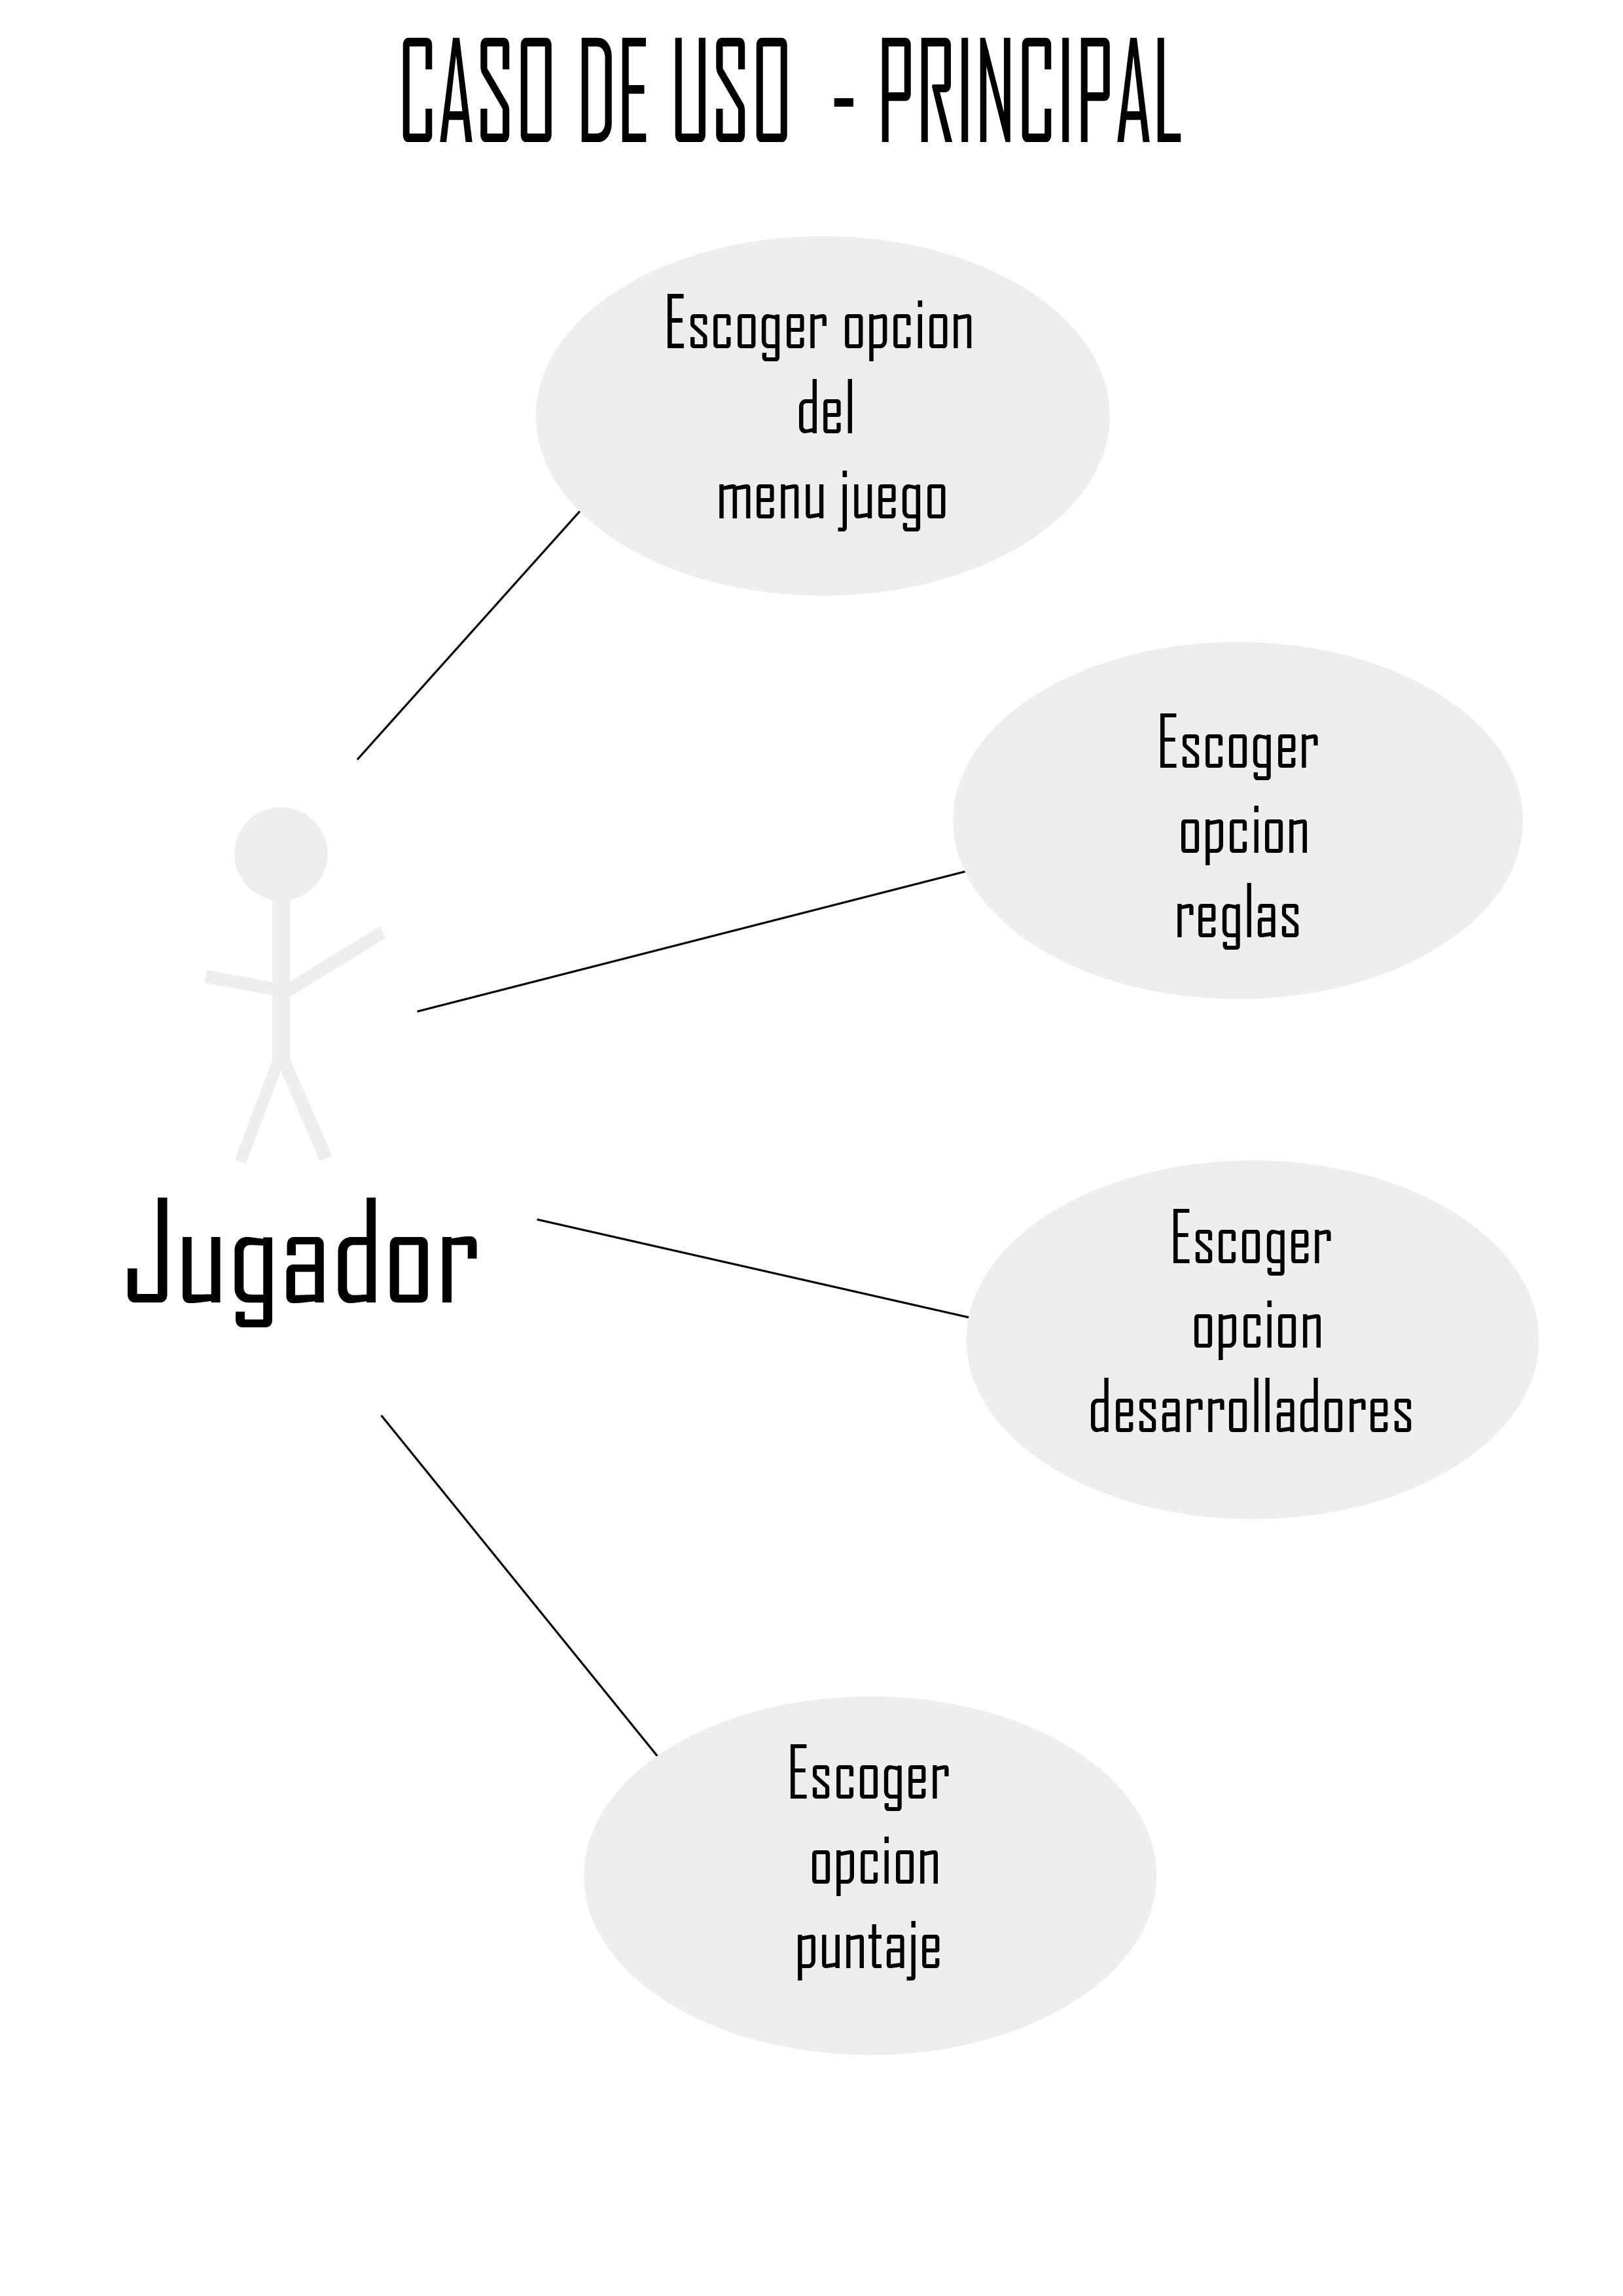
\includegraphics[width=.60\textwidth]{./imagenes/DCU.jpg}
\caption{Diagramas de Casos de usos}
\end{center}
\end{figure}


\chapter{Retroalimientacion}
\include{BuscaminasApp/}

\chapter{Alcance del Proyecto}
En este capitulo trataremos sobre los problemas que encontramos al momento de desarrollar la aplicación y asi mismo como hicimos para resolverlo.

\section{Desarrollo}
Desarrollo del Juego de Buscaminas en Android, implementado para que corra en un TABLE con una versión 3.0.
El juego comienza con la eleccion de 4 acciones:
\newline
\newline
\begin{enumerate}
	\item {Nuevo Juego}
	\item {Puntajes}	
	\item{Reglas}
	\item{Desarroladores}
\end{enumerate}
\begin{figure}[htbp]
\begin{center}
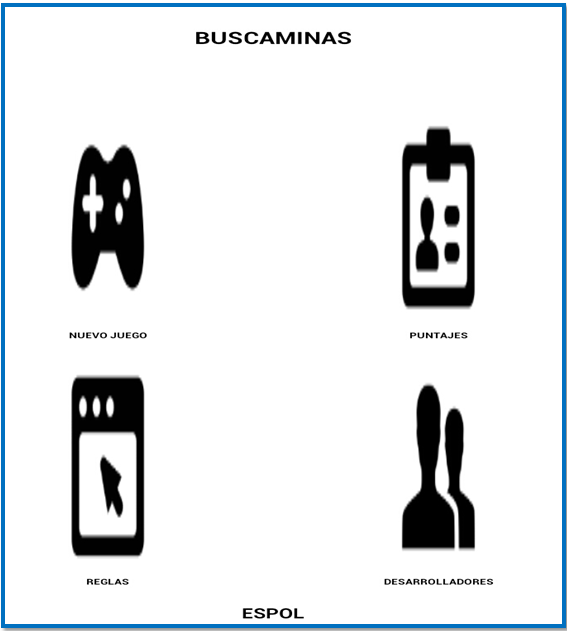
\includegraphics[width=.50\textwidth]{./imagenes/menu.png}
\caption{Menu principal}
\end{center}
Decidimos desarrollar estos botones de una manera diferente, a la convencional, decidimos poner una imagen que identifique a cada accion.
\end{figure}



\begin{figure}[htbp]
\begin{center}
\includegraphics[width=.60\textwidth]{./imagenes/niveles.png}
\caption{Niveles}
\end{center}
Una vez que ingresábamos a NUEVO JUEGO, ingresábamos a esta ventana, que podíamos ingresar el nombre del jugador, el nivel del juego y le dábamos clic en el botón Siguiente.
\end{figure}

\begin{figure}[htbp]
\begin{center}
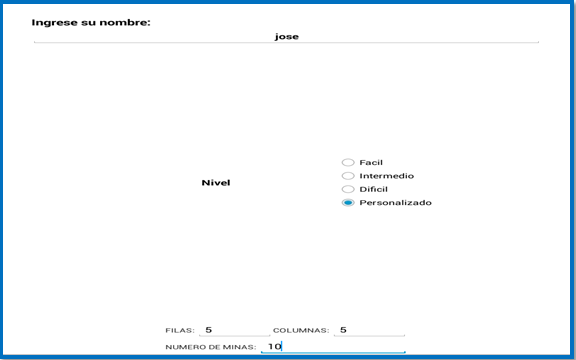
\includegraphics[width=.60\textwidth]{./imagenes/menu2.png}
\caption{Niveles}
\end{center}
deseamos jugar el nivel personalizado, nos aparecerá en la misma ventana 3 campos más; números de filas, números de columnas y el número de bombas para crear una partida personalizada.
\end{figure}
\newpage
AL momento de jugar tendremos 4 niveles:
En estas ventana comenzamos a jugar en los diferentes niveles, y debemos tratar de jugarlo en el menor tiempo posible, para poder estar entre los puntajes más altos del juego, para cada nivel.

\begin{figure}[htbp]
\begin{center}
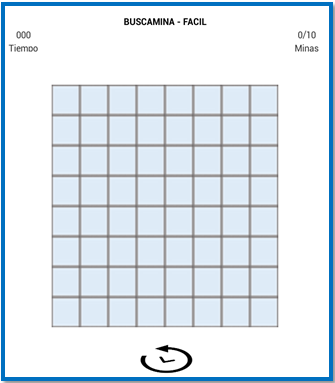
\includegraphics[width=.30\textwidth]{./imagenes/tablero2.png}
\caption{NIVEL FACIL}
\end{center}
Este nivel cuenta con 8x8 celdas, cuenta con 10 minas, también cuenta con el cronometro del tiempo en segundos y cuenta con el botón reiniciar.
\end{figure}

\begin{figure}[htbp]
\begin{center}
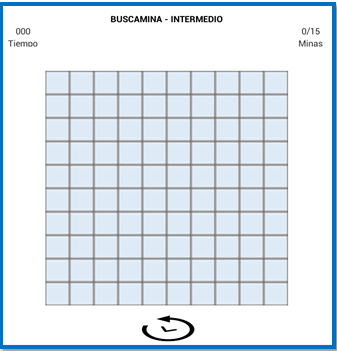
\includegraphics[width=.30\textwidth]{./imagenes/tablero3.png}
\caption{NIVEL INTERMEDIO}
\end{center}
Este nivel cuenta con 10X10 celdas, cuenta con 15 minas, también cuenta con el cronometro del tiempo en segundos y cuenta con el botón reiniciar.
\end{figure}


\begin{figure}[htbp]
\begin{center}
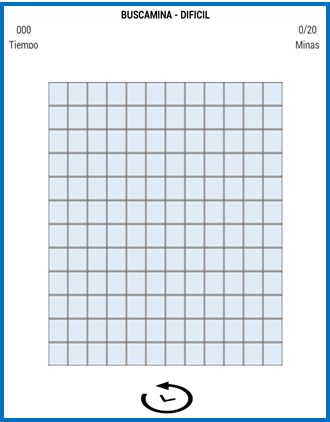
\includegraphics[width=.30\textwidth]{./imagenes/tablero4.png}
\caption{NIVEL DIFICIL}
\end{center}
Este nivel cuenta con 12X12 celdas, cuenta con 20 minas, también cuenta con el cronometro del tiempo en segundos y cuenta con el botón reiniciar.
\end{figure}


\begin{figure}[htbp]
\begin{center}
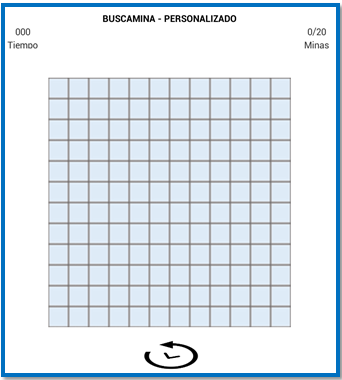
\includegraphics[width=.30\textwidth]{./imagenes/tablero5.png}
\caption{NIVEL PERSONALIZADO}
\end{center}

Este nivel cuenta con que podemos ingresar matrices desde 3x3 hasta 12x12 celdas, cuenta con minas desde 3 minas hasta 143 minas, también cuenta con el cronometro del tiempo en segundos y cuenta con el botón reiniciar.
\end{figure}


\begin{figure}[htbp]
\begin{center}
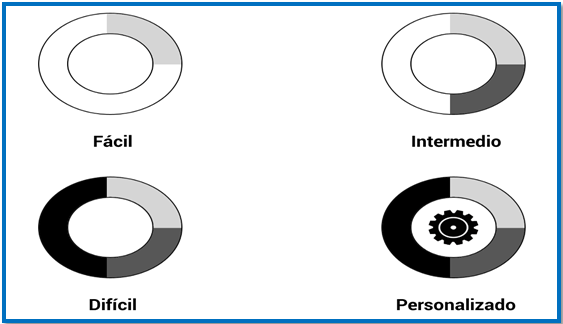
\includegraphics[width=.65\textwidth]{./imagenes/niveles2.png}
\caption{Niveles}
\end{center}

Después por recomendación del profesor, nos pidió que la ventana para elegir los niveles tenga la misma temática del Menú Principal, entras palabras que también tenga n botones que identifique cada acción.
\end{figure}

\begin{figure}[htbp]
\begin{center}
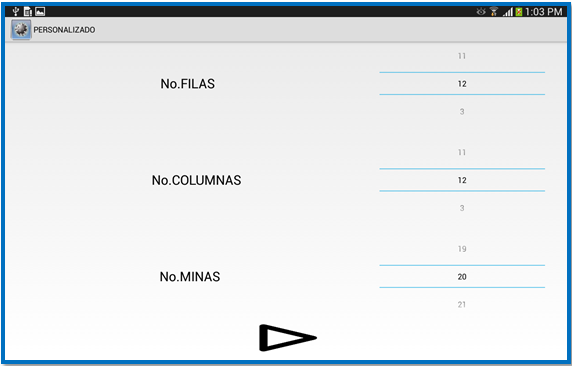
\includegraphics[width=.65\textwidth]{./imagenes/perzonalizado.png}
\caption{Nivel Perzonalizado}
\end{center}
Esta ventana aparecerá si elegimos el nivel personalizado, en donde ingresábamos en nombre y tiempo del jugador.
\end{figure}

\begin{figure}[htbp]
\begin{center}
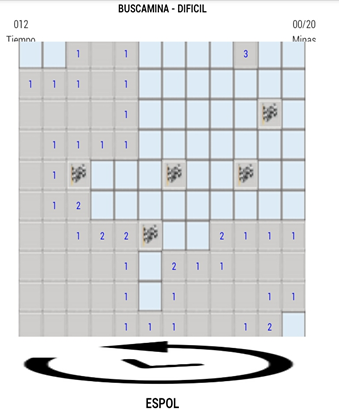
\includegraphics[width=.70\textwidth]{./imagenes/tableroBoton.png}
\caption{Tablero}
\end{center}

Cierto día creamos la bandera en el código, pero al momento de des ocultar una celda que tiene bombas, solo explota loas bombas q esta alrededor de cierta celda.
\end{figure}

\begin{figure}[htbp]
\begin{center}
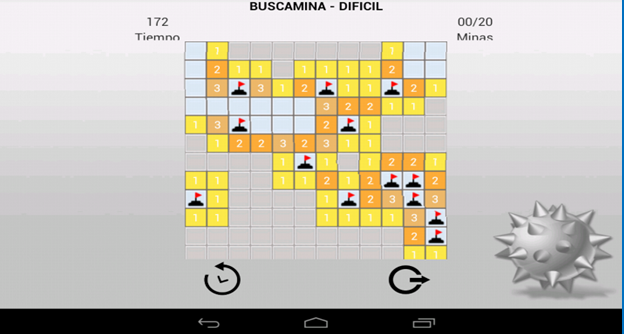
\includegraphics[width=.70\textwidth]{./imagenes/tableroCasilas.png}
\caption{TableroCasillas}
\end{center}

También implementamos que los numero que sale alrededor de otro número, salgas de diferentes colores, para que se pueda ver más colorido.
\end{figure}

\begin{figure}[htbp]
\begin{center}
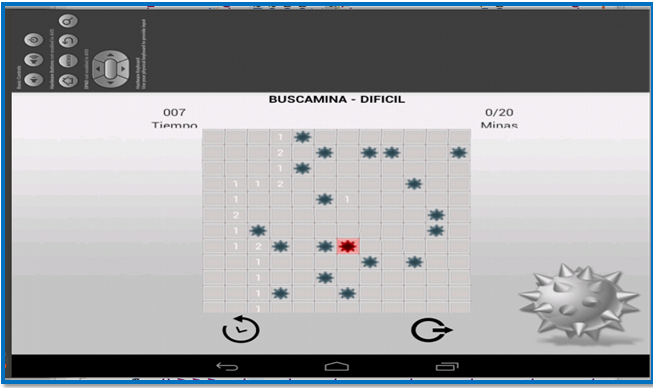
\includegraphics[width=.70\textwidth]{./imagenes/tableroBombas.png}
\caption{TableroBombas}
\end{center}
Aquí también aparecen las bombas encontradas  y la bomba estallada
\end{figure}

\begin{figure}[htbp]
\begin{center}
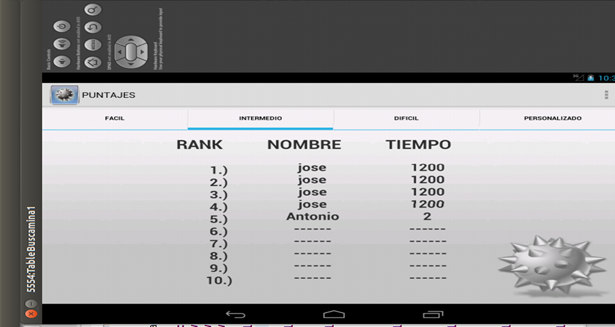
\includegraphics[width=.70\textwidth]{./imagenes/puntajes.png}
\caption{Puntajes}
\end{center}

Por último, si el jugador gana alguna partida, deberá ingresar su nombre y tiempo, y sus datos.
\end{figure}


\chapter{Conclusiones}
\begin{itemize}
\item El lenguaje Android es  muy complicado ya  que trabaja con  Java y XML, a pesar de eso podemos encontrar muchas referencias en la web como google, YouTube y otros paper de referencias.

\item La programación en Android tiene bastante que ver con el diseño de las interfaces en  las aplicaciones,  por tal motivo aprendimos a usar correctamente los distintas formas de layout, para poderlas a usar en las diferentes dimensiones de pantalla. 

\item Comprendimos que el usuario  busca una interfaz sencilla y directa, por el motivo que si existe una relativa cantidad  de ventanas el usuario tiende aburrirse.

\end{itemize}


\end{document}  
